% Created by tikzDevice version 0.12 on 2018-10-15 14:29:17
% !TEX encoding = UTF-8 Unicode
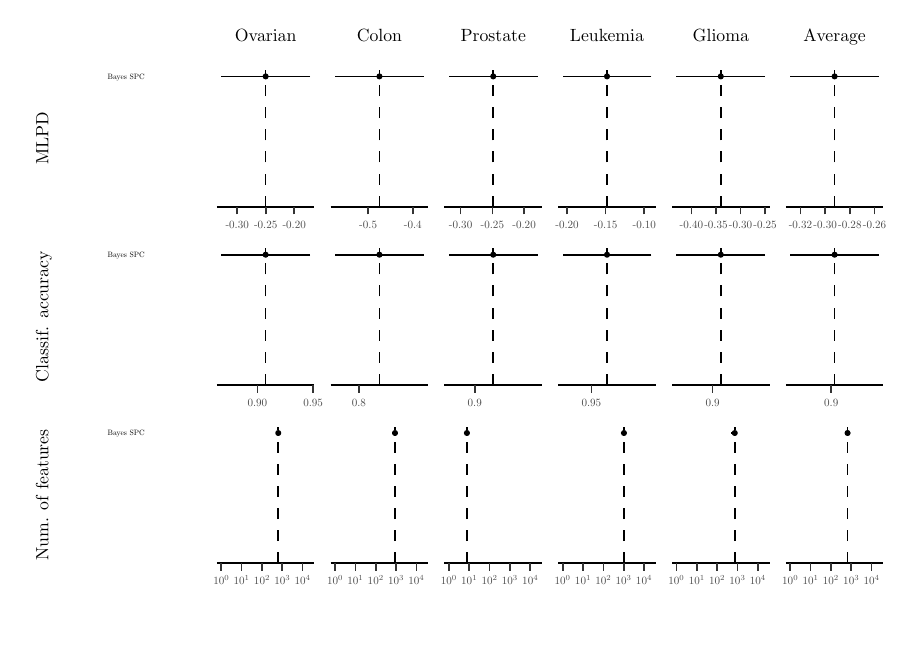
\begin{tikzpicture}[x=1pt,y=1pt]
\definecolor{fillColor}{RGB}{255,255,255}
\path[use as bounding box,fill=fillColor,fill opacity=0.00] (0,0) rectangle (310.76,216.81);
\begin{scope}
\path[clip] (  0.00,204.19) rectangle (  9.80,216.81);
\definecolor{drawColor}{RGB}{255,255,255}
\definecolor{fillColor}{RGB}{255,255,255}

\path[draw=drawColor,line width= 0.6pt,line join=round,line cap=round,fill=fillColor] (  0.00,204.19) rectangle (  9.80,216.81);
\end{scope}
\begin{scope}
\path[clip] (  0.00,139.76) rectangle (  9.80,204.19);
\definecolor{drawColor}{RGB}{255,255,255}
\definecolor{fillColor}{RGB}{255,255,255}

\path[draw=drawColor,line width= 0.6pt,line join=round,line cap=round,fill=fillColor] (  0.00,139.76) rectangle (  9.80,204.19);
\end{scope}
\begin{scope}
\path[clip] (  0.00, 75.32) rectangle (  9.80,139.76);
\definecolor{drawColor}{RGB}{255,255,255}
\definecolor{fillColor}{RGB}{255,255,255}

\path[draw=drawColor,line width= 0.6pt,line join=round,line cap=round,fill=fillColor] (  0.00, 75.32) rectangle (  9.80,139.76);
\end{scope}
\begin{scope}
\path[clip] (  0.00,  0.00) rectangle (  9.80, 75.32);
\definecolor{drawColor}{RGB}{255,255,255}
\definecolor{fillColor}{RGB}{255,255,255}

\path[draw=drawColor,line width= 0.6pt,line join=round,line cap=round,fill=fillColor] (  0.00,  0.00) rectangle (  9.80, 75.32);
\end{scope}
\begin{scope}
\path[clip] (  9.80,204.19) rectangle ( 64.06,216.81);
\definecolor{drawColor}{RGB}{255,255,255}
\definecolor{fillColor}{RGB}{255,255,255}

\path[draw=drawColor,line width= 0.6pt,line join=round,line cap=round,fill=fillColor] (  9.80,204.19) rectangle ( 64.06,216.81);
\end{scope}
\begin{scope}
\path[clip] (  9.80,139.76) rectangle ( 64.06,204.19);
\definecolor{drawColor}{RGB}{255,255,255}
\definecolor{fillColor}{RGB}{255,255,255}

\path[draw=drawColor,line width= 0.6pt,line join=round,line cap=round,fill=fillColor] (  9.80,139.76) rectangle ( 64.06,204.19);
\end{scope}
\begin{scope}
\path[clip] (  9.80, 75.32) rectangle ( 64.06,139.76);
\definecolor{drawColor}{RGB}{255,255,255}
\definecolor{fillColor}{RGB}{255,255,255}

\path[draw=drawColor,line width= 0.6pt,line join=round,line cap=round,fill=fillColor] (  9.80, 75.32) rectangle ( 64.06,139.76);
\end{scope}
\begin{scope}
\path[clip] (  9.80,  0.00) rectangle ( 64.06, 75.32);
\definecolor{drawColor}{RGB}{255,255,255}
\definecolor{fillColor}{RGB}{255,255,255}

\path[draw=drawColor,line width= 0.6pt,line join=round,line cap=round,fill=fillColor] (  9.80,  0.00) rectangle ( 64.06, 75.32);
\end{scope}
\begin{scope}
\path[clip] ( 64.06,204.19) rectangle (105.18,216.81);
\definecolor{drawColor}{RGB}{255,255,255}
\definecolor{fillColor}{RGB}{255,255,255}

\path[draw=drawColor,line width= 0.6pt,line join=round,line cap=round,fill=fillColor] ( 64.06,204.19) rectangle (105.18,216.81);
\end{scope}
\begin{scope}
\path[clip] ( 64.06,139.76) rectangle (105.18,204.19);
\definecolor{drawColor}{RGB}{255,255,255}
\definecolor{fillColor}{RGB}{255,255,255}

\path[draw=drawColor,line width= 0.6pt,line join=round,line cap=round,fill=fillColor] ( 64.06,139.76) rectangle (105.18,204.19);
\end{scope}
\begin{scope}
\path[clip] ( 64.06, 75.32) rectangle (105.18,139.76);
\definecolor{drawColor}{RGB}{255,255,255}
\definecolor{fillColor}{RGB}{255,255,255}

\path[draw=drawColor,line width= 0.6pt,line join=round,line cap=round,fill=fillColor] ( 64.06, 75.32) rectangle (105.18,139.76);
\end{scope}
\begin{scope}
\path[clip] ( 64.06,  0.00) rectangle (105.18, 75.32);
\definecolor{drawColor}{RGB}{255,255,255}
\definecolor{fillColor}{RGB}{255,255,255}

\path[draw=drawColor,line width= 0.6pt,line join=round,line cap=round,fill=fillColor] ( 64.06,  0.00) rectangle (105.18, 75.32);
\end{scope}
\begin{scope}
\path[clip] (105.18,204.19) rectangle (146.29,216.81);
\definecolor{drawColor}{RGB}{255,255,255}
\definecolor{fillColor}{RGB}{255,255,255}

\path[draw=drawColor,line width= 0.6pt,line join=round,line cap=round,fill=fillColor] (105.18,204.19) rectangle (146.29,216.81);
\end{scope}
\begin{scope}
\path[clip] (105.18,139.76) rectangle (146.29,204.19);
\definecolor{drawColor}{RGB}{255,255,255}
\definecolor{fillColor}{RGB}{255,255,255}

\path[draw=drawColor,line width= 0.6pt,line join=round,line cap=round,fill=fillColor] (105.18,139.76) rectangle (146.29,204.19);
\end{scope}
\begin{scope}
\path[clip] (105.18, 75.32) rectangle (146.29,139.76);
\definecolor{drawColor}{RGB}{255,255,255}
\definecolor{fillColor}{RGB}{255,255,255}

\path[draw=drawColor,line width= 0.6pt,line join=round,line cap=round,fill=fillColor] (105.18, 75.32) rectangle (146.29,139.76);
\end{scope}
\begin{scope}
\path[clip] (105.18,  0.00) rectangle (146.29, 75.32);
\definecolor{drawColor}{RGB}{255,255,255}
\definecolor{fillColor}{RGB}{255,255,255}

\path[draw=drawColor,line width= 0.6pt,line join=round,line cap=round,fill=fillColor] (105.18,  0.00) rectangle (146.29, 75.32);
\end{scope}
\begin{scope}
\path[clip] (146.29,204.19) rectangle (187.41,216.81);
\definecolor{drawColor}{RGB}{255,255,255}
\definecolor{fillColor}{RGB}{255,255,255}

\path[draw=drawColor,line width= 0.6pt,line join=round,line cap=round,fill=fillColor] (146.29,204.19) rectangle (187.41,216.81);
\end{scope}
\begin{scope}
\path[clip] (146.29,139.76) rectangle (187.41,204.19);
\definecolor{drawColor}{RGB}{255,255,255}
\definecolor{fillColor}{RGB}{255,255,255}

\path[draw=drawColor,line width= 0.6pt,line join=round,line cap=round,fill=fillColor] (146.29,139.76) rectangle (187.41,204.19);
\end{scope}
\begin{scope}
\path[clip] (146.29, 75.32) rectangle (187.41,139.76);
\definecolor{drawColor}{RGB}{255,255,255}
\definecolor{fillColor}{RGB}{255,255,255}

\path[draw=drawColor,line width= 0.6pt,line join=round,line cap=round,fill=fillColor] (146.29, 75.32) rectangle (187.41,139.76);
\end{scope}
\begin{scope}
\path[clip] (146.29,  0.00) rectangle (187.41, 75.32);
\definecolor{drawColor}{RGB}{255,255,255}
\definecolor{fillColor}{RGB}{255,255,255}

\path[draw=drawColor,line width= 0.6pt,line join=round,line cap=round,fill=fillColor] (146.29,  0.00) rectangle (187.41, 75.32);
\end{scope}
\begin{scope}
\path[clip] (187.41,204.19) rectangle (228.53,216.81);
\definecolor{drawColor}{RGB}{255,255,255}
\definecolor{fillColor}{RGB}{255,255,255}

\path[draw=drawColor,line width= 0.6pt,line join=round,line cap=round,fill=fillColor] (187.41,204.19) rectangle (228.53,216.81);
\end{scope}
\begin{scope}
\path[clip] (187.41,139.76) rectangle (228.53,204.19);
\definecolor{drawColor}{RGB}{255,255,255}
\definecolor{fillColor}{RGB}{255,255,255}

\path[draw=drawColor,line width= 0.6pt,line join=round,line cap=round,fill=fillColor] (187.41,139.76) rectangle (228.53,204.19);
\end{scope}
\begin{scope}
\path[clip] (187.41, 75.32) rectangle (228.53,139.76);
\definecolor{drawColor}{RGB}{255,255,255}
\definecolor{fillColor}{RGB}{255,255,255}

\path[draw=drawColor,line width= 0.6pt,line join=round,line cap=round,fill=fillColor] (187.41, 75.32) rectangle (228.53,139.76);
\end{scope}
\begin{scope}
\path[clip] (187.41,  0.00) rectangle (228.53, 75.32);
\definecolor{drawColor}{RGB}{255,255,255}
\definecolor{fillColor}{RGB}{255,255,255}

\path[draw=drawColor,line width= 0.6pt,line join=round,line cap=round,fill=fillColor] (187.41,  0.00) rectangle (228.53, 75.32);
\end{scope}
\begin{scope}
\path[clip] (228.53,204.19) rectangle (269.64,216.81);
\definecolor{drawColor}{RGB}{255,255,255}
\definecolor{fillColor}{RGB}{255,255,255}

\path[draw=drawColor,line width= 0.6pt,line join=round,line cap=round,fill=fillColor] (228.53,204.19) rectangle (269.64,216.81);
\end{scope}
\begin{scope}
\path[clip] (228.53,139.76) rectangle (269.64,204.19);
\definecolor{drawColor}{RGB}{255,255,255}
\definecolor{fillColor}{RGB}{255,255,255}

\path[draw=drawColor,line width= 0.6pt,line join=round,line cap=round,fill=fillColor] (228.53,139.76) rectangle (269.64,204.19);
\end{scope}
\begin{scope}
\path[clip] (228.53, 75.32) rectangle (269.64,139.76);
\definecolor{drawColor}{RGB}{255,255,255}
\definecolor{fillColor}{RGB}{255,255,255}

\path[draw=drawColor,line width= 0.6pt,line join=round,line cap=round,fill=fillColor] (228.53, 75.32) rectangle (269.64,139.76);
\end{scope}
\begin{scope}
\path[clip] (228.53,  0.00) rectangle (269.64, 75.32);
\definecolor{drawColor}{RGB}{255,255,255}
\definecolor{fillColor}{RGB}{255,255,255}

\path[draw=drawColor,line width= 0.6pt,line join=round,line cap=round,fill=fillColor] (228.53,  0.00) rectangle (269.64, 75.32);
\end{scope}
\begin{scope}
\path[clip] (269.64,204.19) rectangle (310.76,216.81);
\definecolor{drawColor}{RGB}{255,255,255}
\definecolor{fillColor}{RGB}{255,255,255}

\path[draw=drawColor,line width= 0.6pt,line join=round,line cap=round,fill=fillColor] (269.64,204.19) rectangle (310.76,216.81);
\end{scope}
\begin{scope}
\path[clip] (269.64,139.76) rectangle (310.76,204.19);
\definecolor{drawColor}{RGB}{255,255,255}
\definecolor{fillColor}{RGB}{255,255,255}

\path[draw=drawColor,line width= 0.6pt,line join=round,line cap=round,fill=fillColor] (269.64,139.76) rectangle (310.76,204.19);
\end{scope}
\begin{scope}
\path[clip] (269.64, 75.32) rectangle (310.76,139.76);
\definecolor{drawColor}{RGB}{255,255,255}
\definecolor{fillColor}{RGB}{255,255,255}

\path[draw=drawColor,line width= 0.6pt,line join=round,line cap=round,fill=fillColor] (269.64, 75.32) rectangle (310.76,139.76);
\end{scope}
\begin{scope}
\path[clip] (269.64,  0.00) rectangle (310.76, 75.32);
\definecolor{drawColor}{RGB}{255,255,255}
\definecolor{fillColor}{RGB}{255,255,255}

\path[draw=drawColor,line width= 0.6pt,line join=round,line cap=round,fill=fillColor] (269.64,  0.00) rectangle (310.76, 75.32);
\end{scope}
\begin{scope}
\path[clip] (  2.75,206.94) rectangle (  9.80,216.81);
\definecolor{fillColor}{RGB}{255,255,255}

\path[fill=fillColor] (  2.75,206.94) rectangle (  9.80,216.81);
\end{scope}
\begin{scope}
\path[clip] (  2.75,152.11) rectangle (  9.80,201.48);
\definecolor{drawColor}{RGB}{0,0,0}

\node[text=drawColor,rotate= 90.00,anchor=base,inner sep=0pt, outer sep=0pt, scale=  0.64] at (  7.48,176.80) {MLPD};
\end{scope}
\begin{scope}
\path[clip] (  2.75, 87.68) rectangle (  9.80,137.05);
\definecolor{drawColor}{RGB}{0,0,0}

\node[text=drawColor,rotate= 90.00,anchor=base,inner sep=0pt, outer sep=0pt, scale=  0.64] at (  7.48,112.36) {Classif. accuracy};
\end{scope}
\begin{scope}
\path[clip] (  2.75, 23.25) rectangle (  9.80, 72.61);
\definecolor{drawColor}{RGB}{0,0,0}

\node[text=drawColor,rotate= 90.00,anchor=base,inner sep=0pt, outer sep=0pt, scale=  0.64] at (  7.48, 47.93) {Num. of features};
\end{scope}
\begin{scope}
\path[clip] ( 27.25,152.11) rectangle ( 62.51,201.48);
\definecolor{drawColor}{RGB}{0,0,0}

\node[text=drawColor,anchor=base west,inner sep=0pt, outer sep=0pt, scale=  0.28] at ( 28.85,198.22) {Bayes SPC};
\end{scope}
\begin{scope}
\path[clip] ( 27.25, 87.68) rectangle ( 62.51,137.05);
\definecolor{drawColor}{RGB}{0,0,0}

\node[text=drawColor,anchor=base west,inner sep=0pt, outer sep=0pt, scale=  0.28] at ( 28.85,133.79) {Bayes SPC};
\end{scope}
\begin{scope}
\path[clip] ( 27.25, 23.25) rectangle ( 62.51, 72.61);
\definecolor{drawColor}{RGB}{0,0,0}

\node[text=drawColor,anchor=base west,inner sep=0pt, outer sep=0pt, scale=  0.28] at ( 28.85, 69.36) {Bayes SPC};
\end{scope}
\begin{scope}
\path[clip] ( 68.36,206.94) rectangle (103.62,216.81);
\definecolor{drawColor}{RGB}{0,0,0}

\node[text=drawColor,anchor=base,inner sep=0pt, outer sep=0pt, scale=  0.64] at ( 85.99,211.95) {Ovarian};
\end{scope}
\begin{scope}
\path[clip] ( 68.36,152.11) rectangle (103.62,201.48);
\definecolor{fillColor}{RGB}{255,255,255}

\path[fill=fillColor] ( 68.36,152.11) rectangle (103.62,201.48);
\definecolor{drawColor}{RGB}{0,0,0}
\definecolor{fillColor}{RGB}{0,0,0}

\path[draw=drawColor,line width= 0.4pt,line join=round,line cap=round,fill=fillColor] ( 85.99,199.20) circle (  0.89);

\path[draw=drawColor,line width= 0.6pt,line join=round] (102.02,199.20) --
	(102.02,199.20);

\path[draw=drawColor,line width= 0.6pt,line join=round] (102.02,199.20) --
	( 69.97,199.20);

\path[draw=drawColor,line width= 0.6pt,line join=round] ( 69.97,199.20) --
	( 69.97,199.20);

\path[draw=drawColor,line width= 0.6pt,dash pattern=on 4pt off 4pt ,line join=round] ( 85.99,152.11) -- ( 85.99,201.48);
\end{scope}
\begin{scope}
\path[clip] ( 68.36, 87.68) rectangle (103.62,137.05);
\definecolor{fillColor}{RGB}{255,255,255}

\path[fill=fillColor] ( 68.36, 87.68) rectangle (103.62,137.05);
\definecolor{drawColor}{RGB}{0,0,0}
\definecolor{fillColor}{RGB}{0,0,0}

\path[draw=drawColor,line width= 0.4pt,line join=round,line cap=round,fill=fillColor] ( 85.99,134.77) circle (  0.89);

\path[draw=drawColor,line width= 0.6pt,line join=round] (102.02,134.77) --
	(102.02,134.77);

\path[draw=drawColor,line width= 0.6pt,line join=round] (102.02,134.77) --
	( 69.97,134.77);

\path[draw=drawColor,line width= 0.6pt,line join=round] ( 69.97,134.77) --
	( 69.97,134.77);

\path[draw=drawColor,line width= 0.6pt,dash pattern=on 4pt off 4pt ,line join=round] ( 85.99, 87.68) -- ( 85.99,137.05);
\end{scope}
\begin{scope}
\path[clip] ( 68.36, 23.25) rectangle (103.62, 72.61);
\definecolor{fillColor}{RGB}{255,255,255}

\path[fill=fillColor] ( 68.36, 23.25) rectangle (103.62, 72.61);
\definecolor{drawColor}{RGB}{0,0,0}
\definecolor{fillColor}{RGB}{0,0,0}

\path[draw=drawColor,line width= 0.4pt,line join=round,line cap=round,fill=fillColor] ( 90.55, 70.34) circle (  0.89);

\path[draw=drawColor,line width= 0.6pt,line join=round] ( 91.18, 70.34) --
	( 91.18, 70.34);

\path[draw=drawColor,line width= 0.6pt,line join=round] ( 91.18, 70.34) --
	( 89.77, 70.34);

\path[draw=drawColor,line width= 0.6pt,line join=round] ( 89.77, 70.34) --
	( 89.77, 70.34);

\path[draw=drawColor,line width= 0.6pt,dash pattern=on 4pt off 4pt ,line join=round] ( 90.55, 23.25) -- ( 90.55, 72.61);
\end{scope}
\begin{scope}
\path[clip] (109.48,206.94) rectangle (144.74,216.81);
\definecolor{drawColor}{RGB}{0,0,0}

\node[text=drawColor,anchor=base,inner sep=0pt, outer sep=0pt, scale=  0.64] at (127.11,211.95) {Colon};
\end{scope}
\begin{scope}
\path[clip] (109.48,152.11) rectangle (144.74,201.48);
\definecolor{fillColor}{RGB}{255,255,255}

\path[fill=fillColor] (109.48,152.11) rectangle (144.74,201.48);
\definecolor{drawColor}{RGB}{0,0,0}
\definecolor{fillColor}{RGB}{0,0,0}

\path[draw=drawColor,line width= 0.4pt,line join=round,line cap=round,fill=fillColor] (127.11,199.20) circle (  0.89);

\path[draw=drawColor,line width= 0.6pt,line join=round] (143.14,199.20) --
	(143.14,199.20);

\path[draw=drawColor,line width= 0.6pt,line join=round] (143.14,199.20) --
	(111.08,199.20);

\path[draw=drawColor,line width= 0.6pt,line join=round] (111.08,199.20) --
	(111.08,199.20);

\path[draw=drawColor,line width= 0.6pt,dash pattern=on 4pt off 4pt ,line join=round] (127.11,152.11) -- (127.11,201.48);
\end{scope}
\begin{scope}
\path[clip] (109.48, 87.68) rectangle (144.74,137.05);
\definecolor{fillColor}{RGB}{255,255,255}

\path[fill=fillColor] (109.48, 87.68) rectangle (144.74,137.05);
\definecolor{drawColor}{RGB}{0,0,0}
\definecolor{fillColor}{RGB}{0,0,0}

\path[draw=drawColor,line width= 0.4pt,line join=round,line cap=round,fill=fillColor] (127.11,134.77) circle (  0.89);

\path[draw=drawColor,line width= 0.6pt,line join=round] (143.14,134.77) --
	(143.14,134.77);

\path[draw=drawColor,line width= 0.6pt,line join=round] (143.14,134.77) --
	(111.08,134.77);

\path[draw=drawColor,line width= 0.6pt,line join=round] (111.08,134.77) --
	(111.08,134.77);

\path[draw=drawColor,line width= 0.6pt,dash pattern=on 4pt off 4pt ,line join=round] (127.11, 87.68) -- (127.11,137.05);
\end{scope}
\begin{scope}
\path[clip] (109.48, 23.25) rectangle (144.74, 72.61);
\definecolor{fillColor}{RGB}{255,255,255}

\path[fill=fillColor] (109.48, 23.25) rectangle (144.74, 72.61);
\definecolor{drawColor}{RGB}{0,0,0}
\definecolor{fillColor}{RGB}{0,0,0}

\path[draw=drawColor,line width= 0.4pt,line join=round,line cap=round,fill=fillColor] (132.73, 70.34) circle (  0.89);

\path[draw=drawColor,line width= 0.6pt,line join=round] (133.27, 70.34) --
	(133.27, 70.34);

\path[draw=drawColor,line width= 0.6pt,line join=round] (133.27, 70.34) --
	(132.07, 70.34);

\path[draw=drawColor,line width= 0.6pt,line join=round] (132.07, 70.34) --
	(132.07, 70.34);

\path[draw=drawColor,line width= 0.6pt,dash pattern=on 4pt off 4pt ,line join=round] (132.73, 23.25) -- (132.73, 72.61);
\end{scope}
\begin{scope}
\path[clip] (150.60,206.94) rectangle (185.86,216.81);
\definecolor{drawColor}{RGB}{0,0,0}

\node[text=drawColor,anchor=base,inner sep=0pt, outer sep=0pt, scale=  0.64] at (168.23,211.95) {Prostate};
\end{scope}
\begin{scope}
\path[clip] (150.60,152.11) rectangle (185.86,201.48);
\definecolor{fillColor}{RGB}{255,255,255}

\path[fill=fillColor] (150.60,152.11) rectangle (185.86,201.48);
\definecolor{drawColor}{RGB}{0,0,0}
\definecolor{fillColor}{RGB}{0,0,0}

\path[draw=drawColor,line width= 0.4pt,line join=round,line cap=round,fill=fillColor] (168.23,199.20) circle (  0.89);

\path[draw=drawColor,line width= 0.6pt,line join=round] (184.25,199.20) --
	(184.25,199.20);

\path[draw=drawColor,line width= 0.6pt,line join=round] (184.25,199.20) --
	(152.20,199.20);

\path[draw=drawColor,line width= 0.6pt,line join=round] (152.20,199.20) --
	(152.20,199.20);

\path[draw=drawColor,line width= 0.6pt,dash pattern=on 4pt off 4pt ,line join=round] (168.23,152.11) -- (168.23,201.48);
\end{scope}
\begin{scope}
\path[clip] (150.60, 87.68) rectangle (185.86,137.05);
\definecolor{fillColor}{RGB}{255,255,255}

\path[fill=fillColor] (150.60, 87.68) rectangle (185.86,137.05);
\definecolor{drawColor}{RGB}{0,0,0}
\definecolor{fillColor}{RGB}{0,0,0}

\path[draw=drawColor,line width= 0.4pt,line join=round,line cap=round,fill=fillColor] (168.23,134.77) circle (  0.89);

\path[draw=drawColor,line width= 0.6pt,line join=round] (184.25,134.77) --
	(184.25,134.77);

\path[draw=drawColor,line width= 0.6pt,line join=round] (184.25,134.77) --
	(152.20,134.77);

\path[draw=drawColor,line width= 0.6pt,line join=round] (152.20,134.77) --
	(152.20,134.77);

\path[draw=drawColor,line width= 0.6pt,dash pattern=on 4pt off 4pt ,line join=round] (168.23, 87.68) -- (168.23,137.05);
\end{scope}
\begin{scope}
\path[clip] (150.60, 23.25) rectangle (185.86, 72.61);
\definecolor{fillColor}{RGB}{255,255,255}

\path[fill=fillColor] (150.60, 23.25) rectangle (185.86, 72.61);
\definecolor{drawColor}{RGB}{0,0,0}
\definecolor{fillColor}{RGB}{0,0,0}

\path[draw=drawColor,line width= 0.4pt,line join=round,line cap=round,fill=fillColor] (158.72, 70.34) circle (  0.89);

\path[draw=drawColor,line width= 0.6pt,line join=round] (159.03, 70.34) --
	(159.03, 70.34);

\path[draw=drawColor,line width= 0.6pt,line join=round] (159.03, 70.34) --
	(158.37, 70.34);

\path[draw=drawColor,line width= 0.6pt,line join=round] (158.37, 70.34) --
	(158.37, 70.34);

\path[draw=drawColor,line width= 0.6pt,dash pattern=on 4pt off 4pt ,line join=round] (158.72, 23.25) -- (158.72, 72.61);
\end{scope}
\begin{scope}
\path[clip] (191.71,206.94) rectangle (226.97,216.81);
\definecolor{drawColor}{RGB}{0,0,0}

\node[text=drawColor,anchor=base,inner sep=0pt, outer sep=0pt, scale=  0.64] at (209.34,211.95) {Leukemia};
\end{scope}
\begin{scope}
\path[clip] (191.71,152.11) rectangle (226.97,201.48);
\definecolor{fillColor}{RGB}{255,255,255}

\path[fill=fillColor] (191.71,152.11) rectangle (226.97,201.48);
\definecolor{drawColor}{RGB}{0,0,0}
\definecolor{fillColor}{RGB}{0,0,0}

\path[draw=drawColor,line width= 0.4pt,line join=round,line cap=round,fill=fillColor] (209.34,199.20) circle (  0.89);

\path[draw=drawColor,line width= 0.6pt,line join=round] (225.37,199.20) --
	(225.37,199.20);

\path[draw=drawColor,line width= 0.6pt,line join=round] (225.37,199.20) --
	(193.32,199.20);

\path[draw=drawColor,line width= 0.6pt,line join=round] (193.32,199.20) --
	(193.32,199.20);

\path[draw=drawColor,line width= 0.6pt,dash pattern=on 4pt off 4pt ,line join=round] (209.34,152.11) -- (209.34,201.48);
\end{scope}
\begin{scope}
\path[clip] (191.71, 87.68) rectangle (226.97,137.05);
\definecolor{fillColor}{RGB}{255,255,255}

\path[fill=fillColor] (191.71, 87.68) rectangle (226.97,137.05);
\definecolor{drawColor}{RGB}{0,0,0}
\definecolor{fillColor}{RGB}{0,0,0}

\path[draw=drawColor,line width= 0.4pt,line join=round,line cap=round,fill=fillColor] (209.34,134.77) circle (  0.89);

\path[draw=drawColor,line width= 0.6pt,line join=round] (225.37,134.77) --
	(225.37,134.77);

\path[draw=drawColor,line width= 0.6pt,line join=round] (225.37,134.77) --
	(193.32,134.77);

\path[draw=drawColor,line width= 0.6pt,line join=round] (193.32,134.77) --
	(193.32,134.77);

\path[draw=drawColor,line width= 0.6pt,dash pattern=on 4pt off 4pt ,line join=round] (209.34, 87.68) -- (209.34,137.05);
\end{scope}
\begin{scope}
\path[clip] (191.71, 23.25) rectangle (226.97, 72.61);
\definecolor{fillColor}{RGB}{255,255,255}

\path[fill=fillColor] (191.71, 23.25) rectangle (226.97, 72.61);
\definecolor{drawColor}{RGB}{0,0,0}
\definecolor{fillColor}{RGB}{0,0,0}

\path[draw=drawColor,line width= 0.4pt,line join=round,line cap=round,fill=fillColor] (215.46, 70.34) circle (  0.89);

\path[draw=drawColor,line width= 0.6pt,line join=round] (216.03, 70.34) --
	(216.03, 70.34);

\path[draw=drawColor,line width= 0.6pt,line join=round] (216.03, 70.34) --
	(214.77, 70.34);

\path[draw=drawColor,line width= 0.6pt,line join=round] (214.77, 70.34) --
	(214.77, 70.34);

\path[draw=drawColor,line width= 0.6pt,dash pattern=on 4pt off 4pt ,line join=round] (215.46, 23.25) -- (215.46, 72.61);
\end{scope}
\begin{scope}
\path[clip] (232.83,206.94) rectangle (268.09,216.81);
\definecolor{drawColor}{RGB}{0,0,0}

\node[text=drawColor,anchor=base,inner sep=0pt, outer sep=0pt, scale=  0.64] at (250.46,211.95) {Glioma};
\end{scope}
\begin{scope}
\path[clip] (232.83,152.11) rectangle (268.09,201.48);
\definecolor{fillColor}{RGB}{255,255,255}

\path[fill=fillColor] (232.83,152.11) rectangle (268.09,201.48);
\definecolor{drawColor}{RGB}{0,0,0}
\definecolor{fillColor}{RGB}{0,0,0}

\path[draw=drawColor,line width= 0.4pt,line join=round,line cap=round,fill=fillColor] (250.46,199.20) circle (  0.89);

\path[draw=drawColor,line width= 0.6pt,line join=round] (266.49,199.20) --
	(266.49,199.20);

\path[draw=drawColor,line width= 0.6pt,line join=round] (266.49,199.20) --
	(234.43,199.20);

\path[draw=drawColor,line width= 0.6pt,line join=round] (234.43,199.20) --
	(234.43,199.20);

\path[draw=drawColor,line width= 0.6pt,dash pattern=on 4pt off 4pt ,line join=round] (250.46,152.11) -- (250.46,201.48);
\end{scope}
\begin{scope}
\path[clip] (232.83, 87.68) rectangle (268.09,137.05);
\definecolor{fillColor}{RGB}{255,255,255}

\path[fill=fillColor] (232.83, 87.68) rectangle (268.09,137.05);
\definecolor{drawColor}{RGB}{0,0,0}
\definecolor{fillColor}{RGB}{0,0,0}

\path[draw=drawColor,line width= 0.4pt,line join=round,line cap=round,fill=fillColor] (250.46,134.77) circle (  0.89);

\path[draw=drawColor,line width= 0.6pt,line join=round] (266.49,134.77) --
	(266.49,134.77);

\path[draw=drawColor,line width= 0.6pt,line join=round] (266.49,134.77) --
	(234.43,134.77);

\path[draw=drawColor,line width= 0.6pt,line join=round] (234.43,134.77) --
	(234.43,134.77);

\path[draw=drawColor,line width= 0.6pt,dash pattern=on 4pt off 4pt ,line join=round] (250.46, 87.68) -- (250.46,137.05);
\end{scope}
\begin{scope}
\path[clip] (232.83, 23.25) rectangle (268.09, 72.61);
\definecolor{fillColor}{RGB}{255,255,255}

\path[fill=fillColor] (232.83, 23.25) rectangle (268.09, 72.61);
\definecolor{drawColor}{RGB}{0,0,0}
\definecolor{fillColor}{RGB}{0,0,0}

\path[draw=drawColor,line width= 0.4pt,line join=round,line cap=round,fill=fillColor] (255.50, 70.34) circle (  0.89);

\path[draw=drawColor,line width= 0.6pt,line join=round] (256.44, 70.34) --
	(256.44, 70.34);

\path[draw=drawColor,line width= 0.6pt,line join=round] (256.44, 70.34) --
	(254.17, 70.34);

\path[draw=drawColor,line width= 0.6pt,line join=round] (254.17, 70.34) --
	(254.17, 70.34);

\path[draw=drawColor,line width= 0.6pt,dash pattern=on 4pt off 4pt ,line join=round] (255.50, 23.25) -- (255.50, 72.61);
\end{scope}
\begin{scope}
\path[clip] (273.95,206.94) rectangle (309.21,216.81);
\definecolor{drawColor}{RGB}{0,0,0}

\node[text=drawColor,anchor=base,inner sep=0pt, outer sep=0pt, scale=  0.64] at (291.58,211.95) {Average};
\end{scope}
\begin{scope}
\path[clip] (273.95,152.11) rectangle (309.21,201.48);
\definecolor{fillColor}{RGB}{255,255,255}

\path[fill=fillColor] (273.95,152.11) rectangle (309.21,201.48);
\definecolor{drawColor}{RGB}{0,0,0}
\definecolor{fillColor}{RGB}{0,0,0}

\path[draw=drawColor,line width= 0.4pt,line join=round,line cap=round,fill=fillColor] (291.58,199.20) circle (  0.89);

\path[draw=drawColor,line width= 0.6pt,line join=round] (307.60,199.20) --
	(307.60,199.20);

\path[draw=drawColor,line width= 0.6pt,line join=round] (307.60,199.20) --
	(275.55,199.20);

\path[draw=drawColor,line width= 0.6pt,line join=round] (275.55,199.20) --
	(275.55,199.20);

\path[draw=drawColor,line width= 0.6pt,dash pattern=on 4pt off 4pt ,line join=round] (291.58,152.11) -- (291.58,201.48);
\end{scope}
\begin{scope}
\path[clip] (273.95, 87.68) rectangle (309.21,137.05);
\definecolor{fillColor}{RGB}{255,255,255}

\path[fill=fillColor] (273.95, 87.68) rectangle (309.21,137.05);
\definecolor{drawColor}{RGB}{0,0,0}
\definecolor{fillColor}{RGB}{0,0,0}

\path[draw=drawColor,line width= 0.4pt,line join=round,line cap=round,fill=fillColor] (291.58,134.77) circle (  0.89);

\path[draw=drawColor,line width= 0.6pt,line join=round] (307.60,134.77) --
	(307.60,134.77);

\path[draw=drawColor,line width= 0.6pt,line join=round] (307.60,134.77) --
	(275.55,134.77);

\path[draw=drawColor,line width= 0.6pt,line join=round] (275.55,134.77) --
	(275.55,134.77);

\path[draw=drawColor,line width= 0.6pt,dash pattern=on 4pt off 4pt ,line join=round] (291.58, 87.68) -- (291.58,137.05);
\end{scope}
\begin{scope}
\path[clip] (273.95, 23.25) rectangle (309.21, 72.61);
\definecolor{fillColor}{RGB}{255,255,255}

\path[fill=fillColor] (273.95, 23.25) rectangle (309.21, 72.61);
\definecolor{drawColor}{RGB}{0,0,0}
\definecolor{fillColor}{RGB}{0,0,0}

\path[draw=drawColor,line width= 0.4pt,line join=round,line cap=round,fill=fillColor] (296.26, 70.34) circle (  0.89);

\path[draw=drawColor,line width= 0.6pt,line join=round] (296.61, 70.34) --
	(296.61, 70.34);

\path[draw=drawColor,line width= 0.6pt,line join=round] (296.61, 70.34) --
	(295.86, 70.34);

\path[draw=drawColor,line width= 0.6pt,line join=round] (295.86, 70.34) --
	(295.86, 70.34);

\path[draw=drawColor,line width= 0.6pt,dash pattern=on 4pt off 4pt ,line join=round] (296.26, 23.25) -- (296.26, 72.61);
\end{scope}
\begin{scope}
\path[clip] (  0.00,  0.00) rectangle (310.76,216.81);
\definecolor{drawColor}{RGB}{0,0,0}

\path[draw=drawColor,line width= 0.6pt,line join=round] ( 68.36,152.11) --
	(103.62,152.11);
\end{scope}
\begin{scope}
\path[clip] (  0.00,  0.00) rectangle (310.76,216.81);
\definecolor{drawColor}{gray}{0.20}

\path[draw=drawColor,line width= 0.6pt,line join=round] ( 75.71,149.36) --
	( 75.71,152.11);

\path[draw=drawColor,line width= 0.6pt,line join=round] ( 86.01,149.36) --
	( 86.01,152.11);

\path[draw=drawColor,line width= 0.6pt,line join=round] ( 96.31,149.36) --
	( 96.31,152.11);
\end{scope}
\begin{scope}
\path[clip] (  0.00,  0.00) rectangle (310.76,216.81);
\definecolor{drawColor}{gray}{0.30}

\node[text=drawColor,anchor=base,inner sep=0pt, outer sep=0pt, scale=  0.40] at ( 75.71,144.41) {-0.30};

\node[text=drawColor,anchor=base,inner sep=0pt, outer sep=0pt, scale=  0.40] at ( 86.01,144.41) {-0.25};

\node[text=drawColor,anchor=base,inner sep=0pt, outer sep=0pt, scale=  0.40] at ( 96.31,144.41) {-0.20};
\end{scope}
\begin{scope}
\path[clip] (  0.00,  0.00) rectangle (310.76,216.81);
\definecolor{drawColor}{RGB}{0,0,0}

\path[draw=drawColor,line width= 0.6pt,line join=round] ( 68.36, 87.68) --
	(103.62, 87.68);
\end{scope}
\begin{scope}
\path[clip] (  0.00,  0.00) rectangle (310.76,216.81);
\definecolor{drawColor}{gray}{0.20}

\path[draw=drawColor,line width= 0.6pt,line join=round] ( 83.01, 84.93) --
	( 83.01, 87.68);

\path[draw=drawColor,line width= 0.6pt,line join=round] (103.14, 84.93) --
	(103.14, 87.68);
\end{scope}
\begin{scope}
\path[clip] (  0.00,  0.00) rectangle (310.76,216.81);
\definecolor{drawColor}{gray}{0.30}

\node[text=drawColor,anchor=base,inner sep=0pt, outer sep=0pt, scale=  0.40] at ( 83.01, 79.98) {0.90};

\node[text=drawColor,anchor=base,inner sep=0pt, outer sep=0pt, scale=  0.40] at (103.14, 79.98) {0.95};
\end{scope}
\begin{scope}
\path[clip] (  0.00,  0.00) rectangle (310.76,216.81);
\definecolor{drawColor}{RGB}{0,0,0}

\path[draw=drawColor,line width= 0.6pt,line join=round] ( 68.36, 23.25) --
	(103.62, 23.25);
\end{scope}
\begin{scope}
\path[clip] (  0.00,  0.00) rectangle (310.76,216.81);
\definecolor{drawColor}{gray}{0.20}

\path[draw=drawColor,line width= 0.6pt,line join=round] ( 69.97, 20.50) --
	( 69.97, 23.25);

\path[draw=drawColor,line width= 0.6pt,line join=round] ( 77.32, 20.50) --
	( 77.32, 23.25);

\path[draw=drawColor,line width= 0.6pt,line join=round] ( 84.67, 20.50) --
	( 84.67, 23.25);

\path[draw=drawColor,line width= 0.6pt,line join=round] ( 92.01, 20.50) --
	( 92.01, 23.25);

\path[draw=drawColor,line width= 0.6pt,line join=round] ( 99.36, 20.50) --
	( 99.36, 23.25);
\end{scope}
\begin{scope}
\path[clip] (  0.00,  0.00) rectangle (310.76,216.81);
\definecolor{drawColor}{gray}{0.30}

\node[text=drawColor,anchor=base,inner sep=0pt, outer sep=0pt, scale=  0.40] at ( 69.97, 15.55) {$10^0$};

\node[text=drawColor,anchor=base,inner sep=0pt, outer sep=0pt, scale=  0.40] at ( 77.32, 15.55) {$10^1$};

\node[text=drawColor,anchor=base,inner sep=0pt, outer sep=0pt, scale=  0.40] at ( 84.67, 15.55) {$10^2$};

\node[text=drawColor,anchor=base,inner sep=0pt, outer sep=0pt, scale=  0.40] at ( 92.01, 15.55) {$10^3$};

\node[text=drawColor,anchor=base,inner sep=0pt, outer sep=0pt, scale=  0.40] at ( 99.36, 15.55) {$10^4$};
\end{scope}
\begin{scope}
\path[clip] (  0.00,  0.00) rectangle (310.76,216.81);
\definecolor{drawColor}{RGB}{0,0,0}

\path[draw=drawColor,line width= 0.6pt,line join=round] (109.48,152.11) --
	(144.74,152.11);
\end{scope}
\begin{scope}
\path[clip] (  0.00,  0.00) rectangle (310.76,216.81);
\definecolor{drawColor}{gray}{0.20}

\path[draw=drawColor,line width= 0.6pt,line join=round] (123.02,149.36) --
	(123.02,152.11);

\path[draw=drawColor,line width= 0.6pt,line join=round] (139.18,149.36) --
	(139.18,152.11);
\end{scope}
\begin{scope}
\path[clip] (  0.00,  0.00) rectangle (310.76,216.81);
\definecolor{drawColor}{gray}{0.30}

\node[text=drawColor,anchor=base,inner sep=0pt, outer sep=0pt, scale=  0.40] at (123.02,144.41) {-0.5};

\node[text=drawColor,anchor=base,inner sep=0pt, outer sep=0pt, scale=  0.40] at (139.18,144.41) {-0.4};
\end{scope}
\begin{scope}
\path[clip] (  0.00,  0.00) rectangle (310.76,216.81);
\definecolor{drawColor}{RGB}{0,0,0}

\path[draw=drawColor,line width= 0.6pt,line join=round] (109.48, 87.68) --
	(144.74, 87.68);
\end{scope}
\begin{scope}
\path[clip] (  0.00,  0.00) rectangle (310.76,216.81);
\definecolor{drawColor}{gray}{0.20}

\path[draw=drawColor,line width= 0.6pt,line join=round] (119.71, 84.93) --
	(119.71, 87.68);
\end{scope}
\begin{scope}
\path[clip] (  0.00,  0.00) rectangle (310.76,216.81);
\definecolor{drawColor}{gray}{0.30}

\node[text=drawColor,anchor=base,inner sep=0pt, outer sep=0pt, scale=  0.40] at (119.71, 79.98) {0.8};
\end{scope}
\begin{scope}
\path[clip] (  0.00,  0.00) rectangle (310.76,216.81);
\definecolor{drawColor}{RGB}{0,0,0}

\path[draw=drawColor,line width= 0.6pt,line join=round] (109.48, 23.25) --
	(144.74, 23.25);
\end{scope}
\begin{scope}
\path[clip] (  0.00,  0.00) rectangle (310.76,216.81);
\definecolor{drawColor}{gray}{0.20}

\path[draw=drawColor,line width= 0.6pt,line join=round] (111.08, 20.50) --
	(111.08, 23.25);

\path[draw=drawColor,line width= 0.6pt,line join=round] (118.43, 20.50) --
	(118.43, 23.25);

\path[draw=drawColor,line width= 0.6pt,line join=round] (125.78, 20.50) --
	(125.78, 23.25);

\path[draw=drawColor,line width= 0.6pt,line join=round] (133.13, 20.50) --
	(133.13, 23.25);

\path[draw=drawColor,line width= 0.6pt,line join=round] (140.48, 20.50) --
	(140.48, 23.25);
\end{scope}
\begin{scope}
\path[clip] (  0.00,  0.00) rectangle (310.76,216.81);
\definecolor{drawColor}{gray}{0.30}

\node[text=drawColor,anchor=base,inner sep=0pt, outer sep=0pt, scale=  0.40] at (111.08, 15.55) {$10^0$};

\node[text=drawColor,anchor=base,inner sep=0pt, outer sep=0pt, scale=  0.40] at (118.43, 15.55) {$10^1$};

\node[text=drawColor,anchor=base,inner sep=0pt, outer sep=0pt, scale=  0.40] at (125.78, 15.55) {$10^2$};

\node[text=drawColor,anchor=base,inner sep=0pt, outer sep=0pt, scale=  0.40] at (133.13, 15.55) {$10^3$};

\node[text=drawColor,anchor=base,inner sep=0pt, outer sep=0pt, scale=  0.40] at (140.48, 15.55) {$10^4$};
\end{scope}
\begin{scope}
\path[clip] (  0.00,  0.00) rectangle (310.76,216.81);
\definecolor{drawColor}{RGB}{0,0,0}

\path[draw=drawColor,line width= 0.6pt,line join=round] (150.60,152.11) --
	(185.86,152.11);
\end{scope}
\begin{scope}
\path[clip] (  0.00,  0.00) rectangle (310.76,216.81);
\definecolor{drawColor}{gray}{0.20}

\path[draw=drawColor,line width= 0.6pt,line join=round] (156.45,149.36) --
	(156.45,152.11);

\path[draw=drawColor,line width= 0.6pt,line join=round] (167.92,149.36) --
	(167.92,152.11);

\path[draw=drawColor,line width= 0.6pt,line join=round] (179.39,149.36) --
	(179.39,152.11);
\end{scope}
\begin{scope}
\path[clip] (  0.00,  0.00) rectangle (310.76,216.81);
\definecolor{drawColor}{gray}{0.30}

\node[text=drawColor,anchor=base,inner sep=0pt, outer sep=0pt, scale=  0.40] at (156.45,144.41) {-0.30};

\node[text=drawColor,anchor=base,inner sep=0pt, outer sep=0pt, scale=  0.40] at (167.92,144.41) {-0.25};

\node[text=drawColor,anchor=base,inner sep=0pt, outer sep=0pt, scale=  0.40] at (179.39,144.41) {-0.20};
\end{scope}
\begin{scope}
\path[clip] (  0.00,  0.00) rectangle (310.76,216.81);
\definecolor{drawColor}{RGB}{0,0,0}

\path[draw=drawColor,line width= 0.6pt,line join=round] (150.60, 87.68) --
	(185.86, 87.68);
\end{scope}
\begin{scope}
\path[clip] (  0.00,  0.00) rectangle (310.76,216.81);
\definecolor{drawColor}{gray}{0.20}

\path[draw=drawColor,line width= 0.6pt,line join=round] (161.55, 84.93) --
	(161.55, 87.68);
\end{scope}
\begin{scope}
\path[clip] (  0.00,  0.00) rectangle (310.76,216.81);
\definecolor{drawColor}{gray}{0.30}

\node[text=drawColor,anchor=base,inner sep=0pt, outer sep=0pt, scale=  0.40] at (161.55, 79.98) {0.9};
\end{scope}
\begin{scope}
\path[clip] (  0.00,  0.00) rectangle (310.76,216.81);
\definecolor{drawColor}{RGB}{0,0,0}

\path[draw=drawColor,line width= 0.6pt,line join=round] (150.60, 23.25) --
	(185.86, 23.25);
\end{scope}
\begin{scope}
\path[clip] (  0.00,  0.00) rectangle (310.76,216.81);
\definecolor{drawColor}{gray}{0.20}

\path[draw=drawColor,line width= 0.6pt,line join=round] (152.20, 20.50) --
	(152.20, 23.25);

\path[draw=drawColor,line width= 0.6pt,line join=round] (159.55, 20.50) --
	(159.55, 23.25);

\path[draw=drawColor,line width= 0.6pt,line join=round] (166.90, 20.50) --
	(166.90, 23.25);

\path[draw=drawColor,line width= 0.6pt,line join=round] (174.25, 20.50) --
	(174.25, 23.25);

\path[draw=drawColor,line width= 0.6pt,line join=round] (181.60, 20.50) --
	(181.60, 23.25);
\end{scope}
\begin{scope}
\path[clip] (  0.00,  0.00) rectangle (310.76,216.81);
\definecolor{drawColor}{gray}{0.30}

\node[text=drawColor,anchor=base,inner sep=0pt, outer sep=0pt, scale=  0.40] at (152.20, 15.55) {$10^0$};

\node[text=drawColor,anchor=base,inner sep=0pt, outer sep=0pt, scale=  0.40] at (159.55, 15.55) {$10^1$};

\node[text=drawColor,anchor=base,inner sep=0pt, outer sep=0pt, scale=  0.40] at (166.90, 15.55) {$10^2$};

\node[text=drawColor,anchor=base,inner sep=0pt, outer sep=0pt, scale=  0.40] at (174.25, 15.55) {$10^3$};

\node[text=drawColor,anchor=base,inner sep=0pt, outer sep=0pt, scale=  0.40] at (181.60, 15.55) {$10^4$};
\end{scope}
\begin{scope}
\path[clip] (  0.00,  0.00) rectangle (310.76,216.81);
\definecolor{drawColor}{RGB}{0,0,0}

\path[draw=drawColor,line width= 0.6pt,line join=round] (191.71,152.11) --
	(226.97,152.11);
\end{scope}
\begin{scope}
\path[clip] (  0.00,  0.00) rectangle (310.76,216.81);
\definecolor{drawColor}{gray}{0.20}

\path[draw=drawColor,line width= 0.6pt,line join=round] (194.89,149.36) --
	(194.89,152.11);

\path[draw=drawColor,line width= 0.6pt,line join=round] (208.85,149.36) --
	(208.85,152.11);

\path[draw=drawColor,line width= 0.6pt,line join=round] (222.82,149.36) --
	(222.82,152.11);
\end{scope}
\begin{scope}
\path[clip] (  0.00,  0.00) rectangle (310.76,216.81);
\definecolor{drawColor}{gray}{0.30}

\node[text=drawColor,anchor=base,inner sep=0pt, outer sep=0pt, scale=  0.40] at (194.89,144.41) {-0.20};

\node[text=drawColor,anchor=base,inner sep=0pt, outer sep=0pt, scale=  0.40] at (208.85,144.41) {-0.15};

\node[text=drawColor,anchor=base,inner sep=0pt, outer sep=0pt, scale=  0.40] at (222.82,144.41) {-0.10};
\end{scope}
\begin{scope}
\path[clip] (  0.00,  0.00) rectangle (310.76,216.81);
\definecolor{drawColor}{RGB}{0,0,0}

\path[draw=drawColor,line width= 0.6pt,line join=round] (191.71, 87.68) --
	(226.97, 87.68);
\end{scope}
\begin{scope}
\path[clip] (  0.00,  0.00) rectangle (310.76,216.81);
\definecolor{drawColor}{gray}{0.20}

\path[draw=drawColor,line width= 0.6pt,line join=round] (203.71, 84.93) --
	(203.71, 87.68);
\end{scope}
\begin{scope}
\path[clip] (  0.00,  0.00) rectangle (310.76,216.81);
\definecolor{drawColor}{gray}{0.30}

\node[text=drawColor,anchor=base,inner sep=0pt, outer sep=0pt, scale=  0.40] at (203.71, 79.98) {0.95};
\end{scope}
\begin{scope}
\path[clip] (  0.00,  0.00) rectangle (310.76,216.81);
\definecolor{drawColor}{RGB}{0,0,0}

\path[draw=drawColor,line width= 0.6pt,line join=round] (191.71, 23.25) --
	(226.97, 23.25);
\end{scope}
\begin{scope}
\path[clip] (  0.00,  0.00) rectangle (310.76,216.81);
\definecolor{drawColor}{gray}{0.20}

\path[draw=drawColor,line width= 0.6pt,line join=round] (193.32, 20.50) --
	(193.32, 23.25);

\path[draw=drawColor,line width= 0.6pt,line join=round] (200.67, 20.50) --
	(200.67, 23.25);

\path[draw=drawColor,line width= 0.6pt,line join=round] (208.02, 20.50) --
	(208.02, 23.25);

\path[draw=drawColor,line width= 0.6pt,line join=round] (215.36, 20.50) --
	(215.36, 23.25);

\path[draw=drawColor,line width= 0.6pt,line join=round] (222.71, 20.50) --
	(222.71, 23.25);
\end{scope}
\begin{scope}
\path[clip] (  0.00,  0.00) rectangle (310.76,216.81);
\definecolor{drawColor}{gray}{0.30}

\node[text=drawColor,anchor=base,inner sep=0pt, outer sep=0pt, scale=  0.40] at (193.32, 15.55) {$10^0$};

\node[text=drawColor,anchor=base,inner sep=0pt, outer sep=0pt, scale=  0.40] at (200.67, 15.55) {$10^1$};

\node[text=drawColor,anchor=base,inner sep=0pt, outer sep=0pt, scale=  0.40] at (208.02, 15.55) {$10^2$};

\node[text=drawColor,anchor=base,inner sep=0pt, outer sep=0pt, scale=  0.40] at (215.36, 15.55) {$10^3$};

\node[text=drawColor,anchor=base,inner sep=0pt, outer sep=0pt, scale=  0.40] at (222.71, 15.55) {$10^4$};
\end{scope}
\begin{scope}
\path[clip] (  0.00,  0.00) rectangle (310.76,216.81);
\definecolor{drawColor}{RGB}{0,0,0}

\path[draw=drawColor,line width= 0.6pt,line join=round] (232.83,152.11) --
	(268.09,152.11);
\end{scope}
\begin{scope}
\path[clip] (  0.00,  0.00) rectangle (310.76,216.81);
\definecolor{drawColor}{gray}{0.20}

\path[draw=drawColor,line width= 0.6pt,line join=round] (239.84,149.36) --
	(239.84,152.11);

\path[draw=drawColor,line width= 0.6pt,line join=round] (248.71,149.36) --
	(248.71,152.11);

\path[draw=drawColor,line width= 0.6pt,line join=round] (257.58,149.36) --
	(257.58,152.11);

\path[draw=drawColor,line width= 0.6pt,line join=round] (266.45,149.36) --
	(266.45,152.11);
\end{scope}
\begin{scope}
\path[clip] (  0.00,  0.00) rectangle (310.76,216.81);
\definecolor{drawColor}{gray}{0.30}

\node[text=drawColor,anchor=base,inner sep=0pt, outer sep=0pt, scale=  0.40] at (239.84,144.41) {-0.40};

\node[text=drawColor,anchor=base,inner sep=0pt, outer sep=0pt, scale=  0.40] at (248.71,144.41) {-0.35};

\node[text=drawColor,anchor=base,inner sep=0pt, outer sep=0pt, scale=  0.40] at (257.58,144.41) {-0.30};

\node[text=drawColor,anchor=base,inner sep=0pt, outer sep=0pt, scale=  0.40] at (266.45,144.41) {-0.25};
\end{scope}
\begin{scope}
\path[clip] (  0.00,  0.00) rectangle (310.76,216.81);
\definecolor{drawColor}{RGB}{0,0,0}

\path[draw=drawColor,line width= 0.6pt,line join=round] (232.83, 87.68) --
	(268.09, 87.68);
\end{scope}
\begin{scope}
\path[clip] (  0.00,  0.00) rectangle (310.76,216.81);
\definecolor{drawColor}{gray}{0.20}

\path[draw=drawColor,line width= 0.6pt,line join=round] (247.50, 84.93) --
	(247.50, 87.68);
\end{scope}
\begin{scope}
\path[clip] (  0.00,  0.00) rectangle (310.76,216.81);
\definecolor{drawColor}{gray}{0.30}

\node[text=drawColor,anchor=base,inner sep=0pt, outer sep=0pt, scale=  0.40] at (247.50, 79.98) {0.9};
\end{scope}
\begin{scope}
\path[clip] (  0.00,  0.00) rectangle (310.76,216.81);
\definecolor{drawColor}{RGB}{0,0,0}

\path[draw=drawColor,line width= 0.6pt,line join=round] (232.83, 23.25) --
	(268.09, 23.25);
\end{scope}
\begin{scope}
\path[clip] (  0.00,  0.00) rectangle (310.76,216.81);
\definecolor{drawColor}{gray}{0.20}

\path[draw=drawColor,line width= 0.6pt,line join=round] (234.43, 20.50) --
	(234.43, 23.25);

\path[draw=drawColor,line width= 0.6pt,line join=round] (241.78, 20.50) --
	(241.78, 23.25);

\path[draw=drawColor,line width= 0.6pt,line join=round] (249.13, 20.50) --
	(249.13, 23.25);

\path[draw=drawColor,line width= 0.6pt,line join=round] (256.48, 20.50) --
	(256.48, 23.25);

\path[draw=drawColor,line width= 0.6pt,line join=round] (263.83, 20.50) --
	(263.83, 23.25);
\end{scope}
\begin{scope}
\path[clip] (  0.00,  0.00) rectangle (310.76,216.81);
\definecolor{drawColor}{gray}{0.30}

\node[text=drawColor,anchor=base,inner sep=0pt, outer sep=0pt, scale=  0.40] at (234.43, 15.55) {$10^0$};

\node[text=drawColor,anchor=base,inner sep=0pt, outer sep=0pt, scale=  0.40] at (241.78, 15.55) {$10^1$};

\node[text=drawColor,anchor=base,inner sep=0pt, outer sep=0pt, scale=  0.40] at (249.13, 15.55) {$10^2$};

\node[text=drawColor,anchor=base,inner sep=0pt, outer sep=0pt, scale=  0.40] at (256.48, 15.55) {$10^3$};

\node[text=drawColor,anchor=base,inner sep=0pt, outer sep=0pt, scale=  0.40] at (263.83, 15.55) {$10^4$};
\end{scope}
\begin{scope}
\path[clip] (  0.00,  0.00) rectangle (310.76,216.81);
\definecolor{drawColor}{RGB}{0,0,0}

\path[draw=drawColor,line width= 0.6pt,line join=round] (273.95,152.11) --
	(309.21,152.11);
\end{scope}
\begin{scope}
\path[clip] (  0.00,  0.00) rectangle (310.76,216.81);
\definecolor{drawColor}{gray}{0.20}

\path[draw=drawColor,line width= 0.6pt,line join=round] (279.24,149.36) --
	(279.24,152.11);

\path[draw=drawColor,line width= 0.6pt,line join=round] (288.17,149.36) --
	(288.17,152.11);

\path[draw=drawColor,line width= 0.6pt,line join=round] (297.10,149.36) --
	(297.10,152.11);

\path[draw=drawColor,line width= 0.6pt,line join=round] (306.02,149.36) --
	(306.02,152.11);
\end{scope}
\begin{scope}
\path[clip] (  0.00,  0.00) rectangle (310.76,216.81);
\definecolor{drawColor}{gray}{0.30}

\node[text=drawColor,anchor=base,inner sep=0pt, outer sep=0pt, scale=  0.40] at (279.24,144.41) {-0.32};

\node[text=drawColor,anchor=base,inner sep=0pt, outer sep=0pt, scale=  0.40] at (288.17,144.41) {-0.30};

\node[text=drawColor,anchor=base,inner sep=0pt, outer sep=0pt, scale=  0.40] at (297.10,144.41) {-0.28};

\node[text=drawColor,anchor=base,inner sep=0pt, outer sep=0pt, scale=  0.40] at (306.02,144.41) {-0.26};
\end{scope}
\begin{scope}
\path[clip] (  0.00,  0.00) rectangle (310.76,216.81);
\definecolor{drawColor}{RGB}{0,0,0}

\path[draw=drawColor,line width= 0.6pt,line join=round] (273.95, 87.68) --
	(309.21, 87.68);
\end{scope}
\begin{scope}
\path[clip] (  0.00,  0.00) rectangle (310.76,216.81);
\definecolor{drawColor}{gray}{0.20}

\path[draw=drawColor,line width= 0.6pt,line join=round] (290.38, 84.93) --
	(290.38, 87.68);
\end{scope}
\begin{scope}
\path[clip] (  0.00,  0.00) rectangle (310.76,216.81);
\definecolor{drawColor}{gray}{0.30}

\node[text=drawColor,anchor=base,inner sep=0pt, outer sep=0pt, scale=  0.40] at (290.38, 79.98) {0.9};
\end{scope}
\begin{scope}
\path[clip] (  0.00,  0.00) rectangle (310.76,216.81);
\definecolor{drawColor}{RGB}{0,0,0}

\path[draw=drawColor,line width= 0.6pt,line join=round] (273.95, 23.25) --
	(309.21, 23.25);
\end{scope}
\begin{scope}
\path[clip] (  0.00,  0.00) rectangle (310.76,216.81);
\definecolor{drawColor}{gray}{0.20}

\path[draw=drawColor,line width= 0.6pt,line join=round] (275.55, 20.50) --
	(275.55, 23.25);

\path[draw=drawColor,line width= 0.6pt,line join=round] (282.90, 20.50) --
	(282.90, 23.25);

\path[draw=drawColor,line width= 0.6pt,line join=round] (290.25, 20.50) --
	(290.25, 23.25);

\path[draw=drawColor,line width= 0.6pt,line join=round] (297.60, 20.50) --
	(297.60, 23.25);

\path[draw=drawColor,line width= 0.6pt,line join=round] (304.95, 20.50) --
	(304.95, 23.25);
\end{scope}
\begin{scope}
\path[clip] (  0.00,  0.00) rectangle (310.76,216.81);
\definecolor{drawColor}{gray}{0.30}

\node[text=drawColor,anchor=base,inner sep=0pt, outer sep=0pt, scale=  0.40] at (275.55, 15.55) {$10^0$};

\node[text=drawColor,anchor=base,inner sep=0pt, outer sep=0pt, scale=  0.40] at (282.90, 15.55) {$10^1$};

\node[text=drawColor,anchor=base,inner sep=0pt, outer sep=0pt, scale=  0.40] at (290.25, 15.55) {$10^2$};

\node[text=drawColor,anchor=base,inner sep=0pt, outer sep=0pt, scale=  0.40] at (297.60, 15.55) {$10^3$};

\node[text=drawColor,anchor=base,inner sep=0pt, outer sep=0pt, scale=  0.40] at (304.95, 15.55) {$10^4$};
\end{scope}
\end{tikzpicture}
